\documentclass{article}
\usepackage{caption}
\usepackage{subcaption}
\usepackage{hyperref}
\usepackage{csquotes}
\usepackage{algorithm}
\usepackage{algpseudocode}

\usepackage{parskip}

\hypersetup{
    colorlinks=true,
    linkcolor=blue,
    filecolor=magenta,      
    urlcolor=cyan,
    pdftitle={Wordcrossing Level Generation},
    pdfpagemode=FullScreen,
}

\usepackage{graphicx}
\graphicspath{ {./images/} }

\title{Wordcrossing Level Generation}
\author{Harry Keightley}
\date{\today}

\begin{document}
\maketitle

\section{Background}
\href{https://wordcrossing.com}{Wordcrossing} 
is a little game I made in a weekend, just after wordle blew up in 2023.
It's a little blend of crosswords/scrabble and wordle, where the game is essentially:
\begin{center}
  Given a start and goal position on a 2D grid, and a set of letters, 
  construct a series of valid english words that connects the start and goal positions.
  \vspace{\baselineskip}


\end{center}

\begin{figure}[h]
\centering
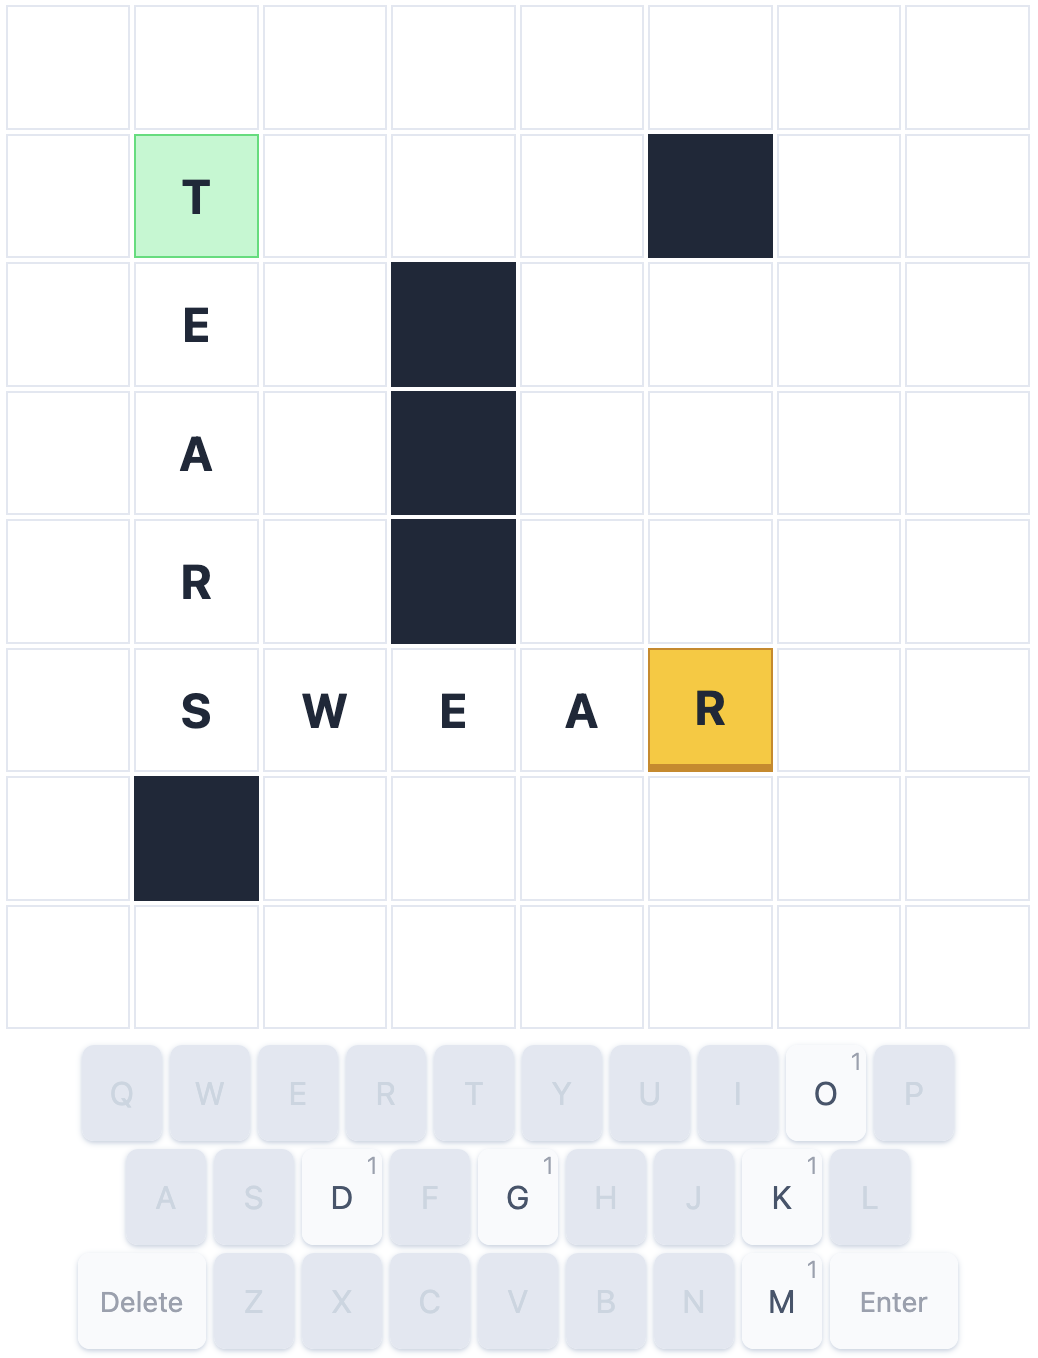
\includegraphics[width=0.5\textwidth]{wc-basic.png}
\caption{Example of a solved wordcrossing}
\label{fig:wc-solved}
\end{figure}

In figure \ref{fig:wc-solved}: 
the start position is the green square;
the goal position is the yellow square; 
and the letters at the bottom of the screen + "tearswear" 
form the total letters that can be used to form solutions.

In the online version of wordcrossing, 
players are incentivised to find a solution that maximises the total letters,
and minimises the number of words placed. This leads to a situation where 
players (being myself, my partner, and my mother), will iterate on their 
solution a few times to compete with eachother. 

If the daily levels are too hard, or even too easy (figure \ref{fig:test}),
it has a big impact on player fun--- turning the level into a slog or a let down, respectively.
Suffice it to say, finding that right balance of difficulty is an important problem to solve for this game, and a
surprisingly fun little task.

\vspace{\baselineskip}
I tend to use wordcrossing.com as a staging area to test new technologies I'm interested in, 
so I have previously written this level generation library in:
\begin{itemize}
  \item Python, when the project was first created, 
    running in a container on Google Cloud, invoked on a cron job,
    where it would write the output to a bucket.
  \item Typescript, when I created a monorepo for generation and playing the game, 
    and to reuse the types between frontend and backend. In this iteration, I used 
    cloudflares functions and workflows for the same functionality as GCP.
  \item And now, Rust, to speed up the level generation process. Depending on our criteria 
    in generating levels, small tweaks can make large differences in runtime, and I was 
    frequently getting time-outs in the typescript implementation. Using rust is also 
    a great excuse to use rust.
  
\end{itemize}

%% Level difficulty figures
\begin{figure}
\centering
\begin{subfigure}{.5\textwidth}
  \centering
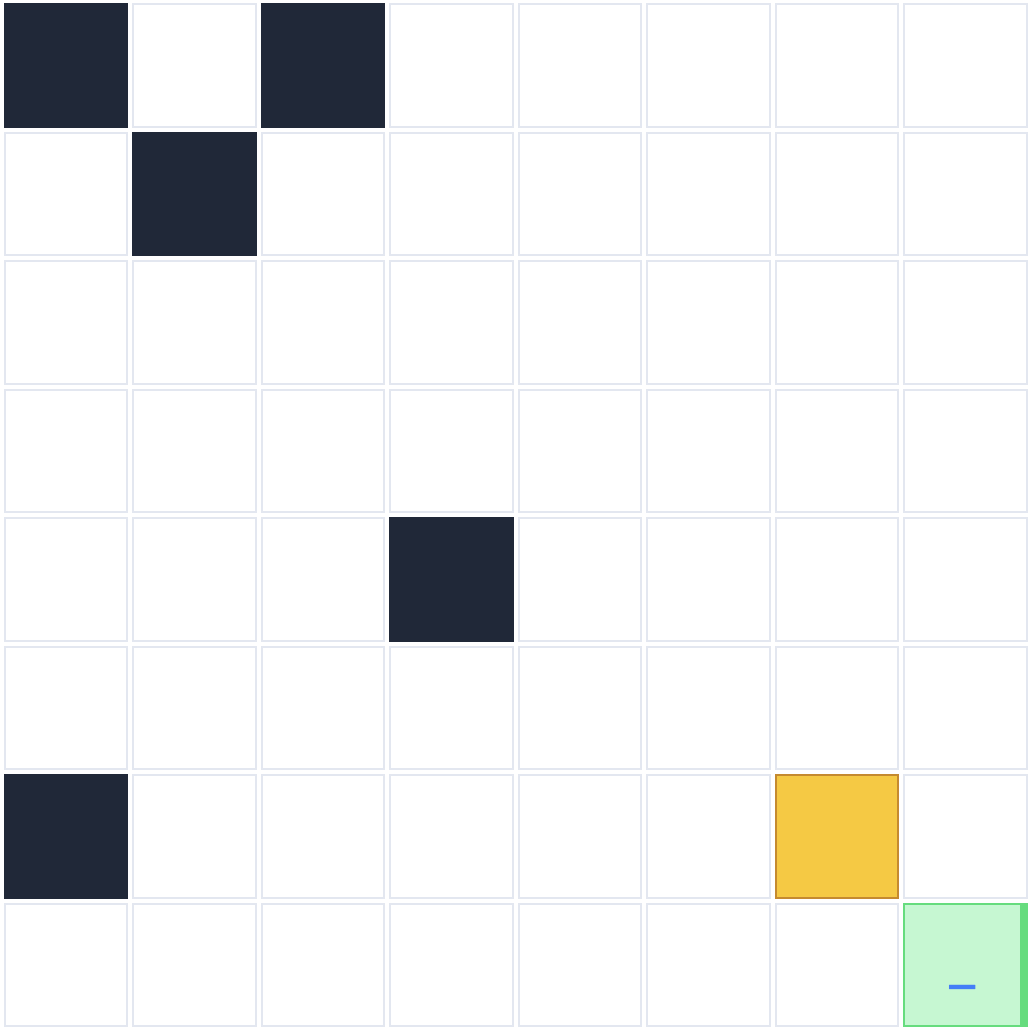
\includegraphics[width=0.8\linewidth]{level-easy.png}
\caption{Too easy}
\label{fig:level-easy}
\end{subfigure}%
\begin{subfigure}{.5\textwidth}
  \centering
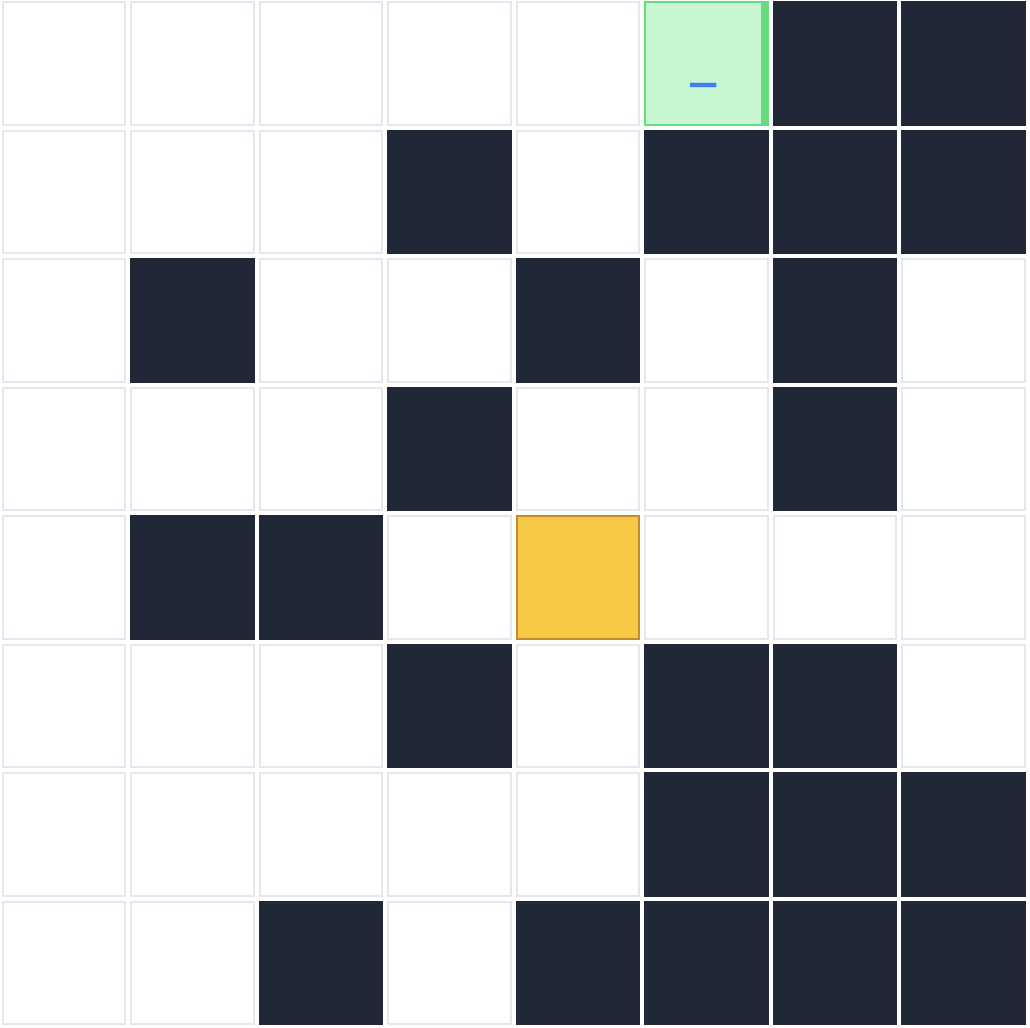
\includegraphics[width=0.8\linewidth]{level-hard.png}
\caption{Too hard}
\label{fig:level-hard}
\end{subfigure}
\caption{Showing differences in level difficulty}
\label{fig:test}
\end{figure}

\newpage

\section{Definitions}
Before we jump into the level generation process, it would be good to have
some common ground for terminology.

\subsection*{Position}
A tuple of integers, (row, column).

\subsection*{Neighbours}
The neighbours of a position are those directly up, down, left and right of it.

\subsection*{Entity (Wall)}
In the level generation part of wordcrossing, the only relevant 
entity is the \texttt{Wall} entity, which is impassable, meaning you 
cannot place letters atop it.

\subsection*{Grid}
A 2D grid of a given rows and columns. Contains entities.

\subsection*{Free space}
The free space in the Grid is the set of positions that aren't Wall entities.

\subsection*{Rooms}
A room, $R$ in the grid is the maximal set of positions such that for any two 
positions, $a, b \in R$, there exists a path in the free space, $[p_0, p_1 ... , p_{n}]$ where:
\begin{itemize}
  \item $a=p_0$
  \item $b=p_n$
  \item For $i \in [1..n]$, $p_i$ neighbours $p_{i-1}$.
\end{itemize}
Maximal here means no more positions can be added to $R$ and have the above hold, i.e. a room is
entirely bordered by walls, or the edge of the bounding grid.

\subsection*{Level}
A Level is a struct of:
\begin{itemize}
  \item A grid.
  \item A start and goal position on the grid.
  \item A HashMap of letters to their counts that could be used to construct words.
\end{itemize}

A level is valid iff:
\begin{itemize}
  \item There exists a room in the grid such that the start and goal are in the room.
  \item The set of letters can be used to create a valid solution from the start to the goal.
\end{itemize}


\section{Level Generation}
A very informal summary of my level generation solution is as follows:

Setup:
\begin{enumerate}
  \item Initialise an empty Grid of the given dimensions.
  \item Setting up some initial walls.
  \item Find all rooms in the grid.
  \item Wall off every room except the biggest one.
  \item Generate a distance map and turn map of the level.
  \item Choose a start and goal position in this room, based on some metrics.
  \item Create a level with an empty letter count.
  \item Iteratively build up words from the start to the goal, based on the
    shortest path to the goal.
\end{enumerate}

Let's dig into some of those in more depth.

\subsection{Initial Walls}
We randomly choose some percentage (between 15\% and 50\%) of positions in the grid
to wall off. This gives a bit more variety to the level. 

\subsection{Exploration}
Exploration--- building rooms within the Grid, is done by calling DFS on each
position in the free space (if we haven't already seen it during one of the last
rooms DFS.

\subsection{Final Walling}
The initial walling both looks jagged, and makes it less clear to the player 
which positions they can validly reach from the start and goal. Walling off the 
unreachable positions in the level fix this.

To do so, we simply choose every room in the grid except the largest, 
and fill it with walls.

\subsection{Distance and Turn Mapping}
For future metrics, it's important to know how far every square is away from 
eachother (governing word length), and how many turns are required to get there 
(governing the number of words in the solution). 

We generate distance and turn maps through Djikstras algorithm.

\subsubsection{Distance Map}
For the distance map, this is 
\href{https://en.wikipedia.org/wiki/Dijkstra%27s_algorithm}{Djikstras}(note: maybe not?),
but calculating minimum distance between any two points in the graph.

In this version, the free space positions are nodes in the graph, with
edges only existing between neighbours, 
and the weight of each edge being 1.

Basically, we initialise an edge map, $E=(position \rightarrow position \rightarrow distance)$
with $E(v, v) = 0$ for each vertex $v$ in the graph.

Then we continue to iterate the graph until it converges, asking:
\begin{algorithm}
\caption{Finding smallest distances between all positions}\label{alg:distance-map}
\begin{algorithmic}
\State{changed} $\gets true$
\While{changed}
  \State{changed} $\gets false$
  \ForAll{position}
    \For{neighbour of position}
      \For{destination in keys(dist(neighbour))}
          \State $d_n \gets 1 + dist(neighbour, destination)$

        \If{$d_n < dist(position, destination)$}
          \State $dist(position, destination) \gets d_n$
          \State $changed \gets true$
        \EndIf
    \EndFor
  \EndFor
  \EndFor
\EndWhile
\end{algorithmic}
\end{algorithm}

There are a few ways to improve the algorithm itself, though who doesn't love 4
separate tiers of nested loops? One idea (alg \ref{alg:distance-map-2} to use a queue to store nodes who have the 
potential to change, instead of just iterating through all nodes each loop. The idea 
there is that we only have to recalculate the distance map for a position when one of its 
neighbours have new information.

\begin{algorithm}
\caption{Finding smallest distances between all positions v2}\label{alg:distance-map-2}
\begin{algorithmic}
\State{changed} $\gets Queue<Position>()$
\State{queued} $\gets Set<Position>()$
\State{dist} $\gets EdgeMap<int>()$
\\

\ForAll{position in FreeSpace}
  \State{changed.enqueue(position)}
  \State{queued.add(position)}
  \State{dist(position, position) $\gets 0$}
\EndFor
\\

\While{!changed.isEmpty()}
  \State{position $\gets$ changed.dequeue()}
  \State{queued.remove(position)}
  \For{neighbour of position}
    \For{destination in keys(dist(neighbour))}
        \State $d_n \gets 1 + dist(neighbour, destination)$

      \If{$d_n < dist(position, destination)$}
        \State $dist(position, destination) \gets d_n$
        \If{!queued.contains(neighbour)}
          \State{queued.add(neighbour)}
          \State{changed.enqueue(neighbour)}
        \EndIf
      \EndIf
    \EndFor
  \EndFor
\EndWhile
\end{algorithmic}
\end{algorithm}

In hindsight (and too late to change for this meetup), we also don't really need this 
distance information between any two points, as this was a hangover from an earlier
iteration of the level generation algorithm. Instead we just need the distances from 
the start (after we randomly choose it) to every other position. Oh well. 

A more interesting idea, probably just because I've never encountered it before, 
is using roughly the same algorithm to make a turn map. In this algorithm, 
instead of storing distance to the goal, we store:
\begin{enumerate}
  \item The number of turns to the goal
  \item The next direction you would need to head in to get there.
\end{enumerate}

The algorithm changes as follows:
\begin{algorithm}
\caption{Finding smallest turns between each position}\label{alg:turn-map}
\begin{algorithmic}
\State{changed} $\gets Queue<Position>()$
\State{queued} $\gets Set<Position>()$
\State{turns} $\gets EdgeMap<(int, Option<Direction>)>()$ 
\Comment (1)
\\

\ForAll{position in FreeSpace}
  \State{changed.enqueue(position)}
  \State{queued.add(position)}
  \State{turns(position, position) $\gets (0, None)$}
\EndFor
\\

\While{!changed.isEmpty()}
  \State{position $\gets$ changed.dequeue()}
  \State{queued.remove(position)}
  \For{neighbour of position}
    \For{destination in keys(turns(neighbour))}
      \State $(turns_n, direction_n) \gets turns(neighbour, destination)$
      \If{position.direction\_to(neighbour) $!=$ $direction_n$}
        \Comment (2)
        \State{$turns_n \gets turns_n + 1$}
      \EndIf

      \If{$turns_n < turns(position, destination)[0]$}
        \State $updated \gets(turns_n, position.direction\_to(neighbour))$
        \State $turns(position, destination) \gets updated$
        \If{!queued.contains(neighbour)}
          \State{queued.add(neighbour)}
          \State{changed.enqueue(neighbour)}
        \EndIf
      \EndIf
    \EndFor
  \EndFor
\EndWhile
\end{algorithmic}
\end{algorithm}

Notes:
\begin{enumerate}
  \item The direction from a position to itself is none in this case.
  \item We only increase the turns if the direction from the neighbour to their destination
    is not the direction from the position to its neighbour.
\end{enumerate}


\subsection{Choosing a Start and Goal}
Now with our distance and turn map, we have everything we need (and more), to choose the 
start and goal positions. Since we've walled off every room except the largest, we know 
all positions in the freespace are reachable from eachother. We can then pick any two 
positions in this space for the start and goal positions.

\begin{enumerate}
  \item We start by randomly selecting a start position from the free space.
  \item In selecting a goal, to make sure we don't pick positions that are too close, 
    or with too many turns, 
    we first sort all candidates ($FreeSpace - start$) in descending order of the sum of:
    \begin{itemize}
      \item Their distance from the start.
      \item And the thir number of turns from the start.
    \end{itemize}
  \item We then select a goal randomly from the first third of the sorted candidates.
\end{enumerate}

\begin{figure}
\centering
\begin{subfigure}{0.2\textwidth}
  \centering
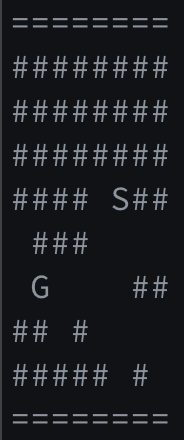
\includegraphics[width=0.8\linewidth]{sg-1.png}
\end{subfigure}%
\begin{subfigure}{0.2\textwidth}
  \centering
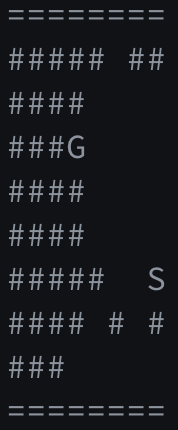
\includegraphics[width=0.8\linewidth]{sg-2.png}
\end{subfigure}
\begin{subfigure}{0.2\textwidth}
  \centering
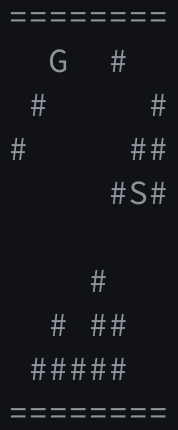
\includegraphics[width=0.8\linewidth]{sg-3.png}
\end{subfigure}
\begin{subfigure}{0.2\textwidth}
  \centering
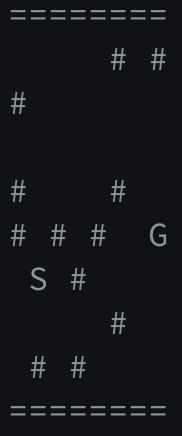
\includegraphics[width=0.8\linewidth]{sg-4.png}
\end{subfigure}
\caption{Start and goal choices}
\label{fig:start-and-goal}
\end{figure}

Figure \ref{fig:start-and-goal} includes a few generated maps, to get a feel for this.
Note that the furthest distances from the start are not always interesting. 

Now that we have our map, and our start and goal positions, it's time to try 
and find a solution!

\subsection{Solving for a Level}
To find a solution for our new level, we start by tracing a minimum turn path 
from the start to the goal node, with the help of our turn map. Note that 
the minimum turns path is always the minimum distance path to the goal, 
with the set of minimum-turn paths between start and goal 
being a subset of the minimum distance
paths (See figure \ref{fig:min-turns-vs-min-distances}).

\begin{figure}
\centering
\begin{subfigure}{0.5\textwidth}
  \centering
  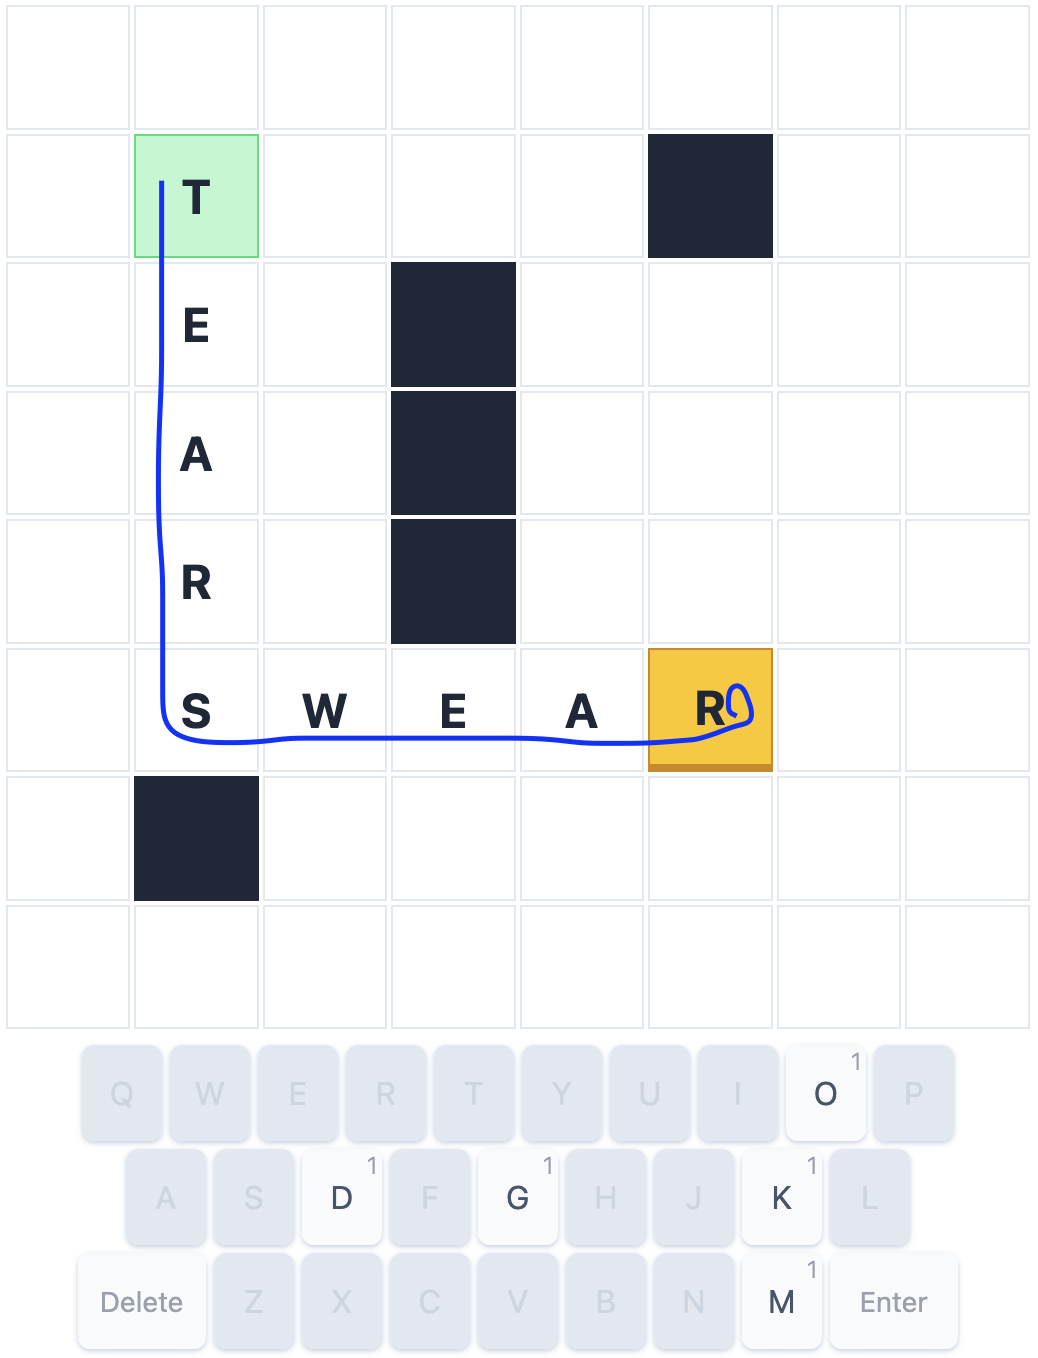
\includegraphics[width=0.8\linewidth]{min-turns.png}
  \subcaption{The minimum turns solution}
\end{subfigure}%
\begin{subfigure}{0.5\textwidth}
  \centering
  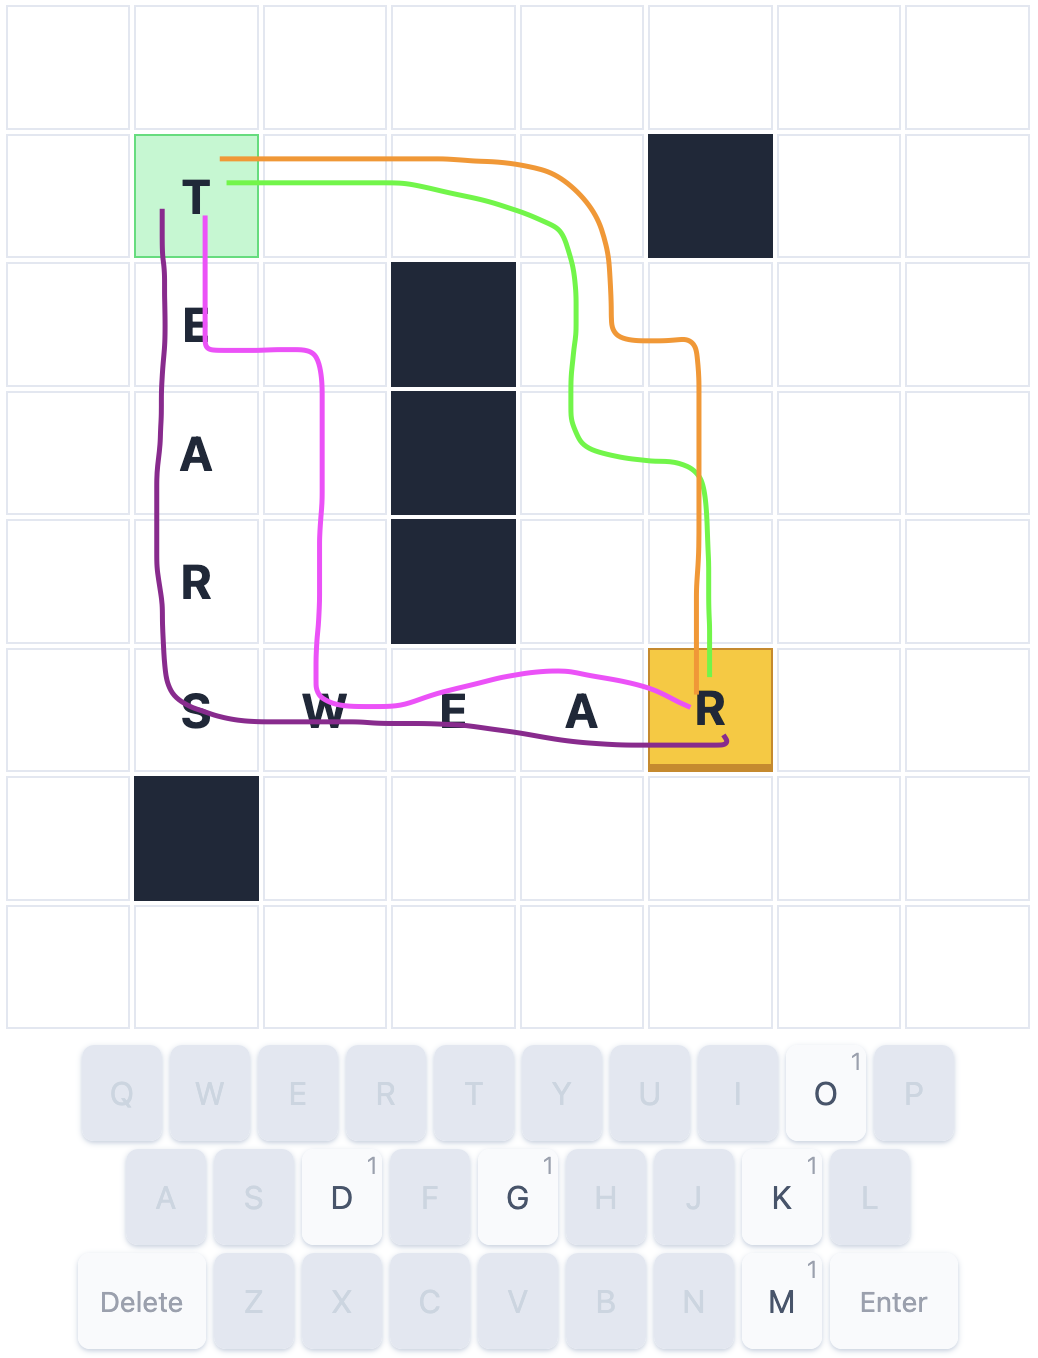
\includegraphics[width=0.8\linewidth]{min-dist.png}
  \subcaption{Some min-distance solutions}
\end{subfigure}
\caption{Comparing solutions}
\label{fig:min-turns-vs-min-distances}
\end{figure}

Next, we convert this path to a series of junctions $(j_0, j_1, ..., j_n)$, between which we will
place our words (figure \ref{fig:junctions}).

\begin{figure}
\centering
  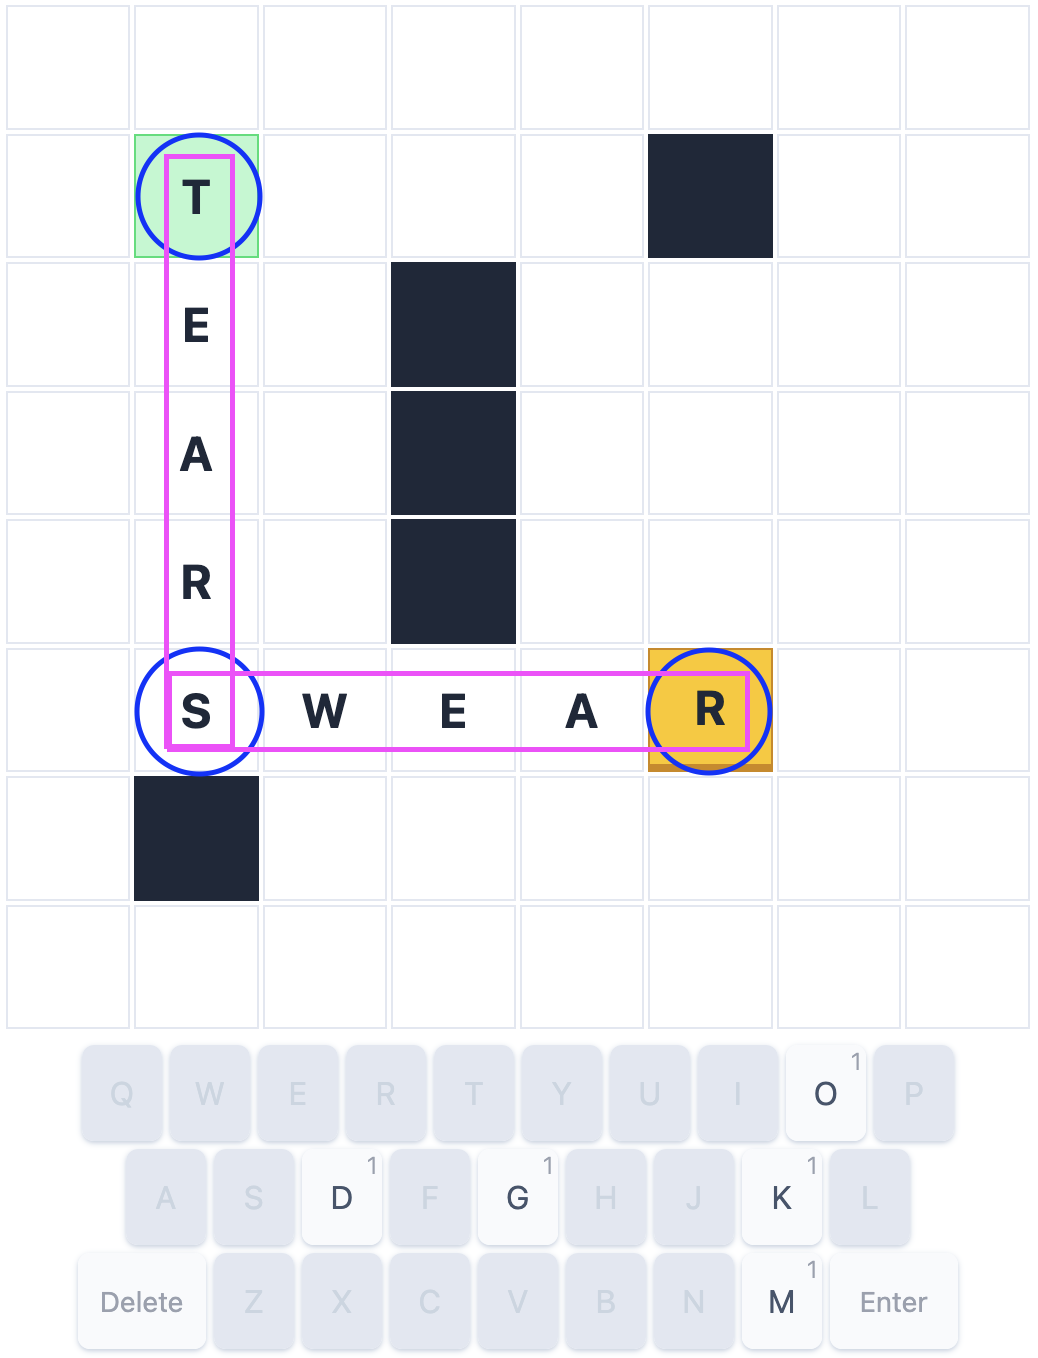
\includegraphics[width=0.4\linewidth]{sol-junctions.png}
\caption{Finding junctions (blue circles), and placing words (purple rects).}
\label{fig:junctions}
\end{figure}

We can then transform our problem of finding a solution, to successively finding
words in our wordlist that satisfy a set of constraints. 
When we have no words in our solution so far, we attempt 
to place a word between the junctions (positions), $j_0$ and $j_1$, with the
only constraint being that the word must have length: $dist(j_0, j_1) + 1$.

For the next word, we have a similar constraint: $length = dist(j_1, j_2) + 1$, 
but we additionally have the constraint that the first letter of this word must 
be the last letter of the previous word. I've called this an "index" constraint in the 
code. This index constraint doesn't always line up the way I've just described.
In wordcrossing, a valid english word can only be placed from left to right,
and from top to bottom. This means that sometimes, the previous word puts an index 
constraint on the \emph{last} letter in the new word 
(imagine switching the start and goal positions in figure \ref{fig:junctions}).

We continue to place words until we've either created a solution that connects the 
start and goal, or we've determined no solution exists given the previous used words. 

There are a number of technical decisions here to address, here which I will
cover in the next sections.

\subsubsection{Wordlist choice}
The choice of the wordlist here can greatly affect how easily players reach a solution.
I use an "easy" wordlist for level generation, and a more permissive wordlist when
you're actually playing the game.

If we choose a permissive wordlist for level generation, it can come up with solutions 
containing words that no (modern) human would understand, which can make the day's 
letters perplexing when you're given an odd combination of "x, z, q, i, and w".

The wordlists for generation and playing the game are supplied in the \texttt{assets}
folder for this repository.

\subsubsection{Wordlist Data Structure}
We want to make word lookups efficient for:
\begin{itemize}
  \item Length lookups
  \item First letter lookups
  \item Last letter lookups
\end{itemize}
One potential choice here would be to have two Maps of:
\begin{displaymath}
  WordLength \rightarrow StartLetter \rightarrow Set<Word>
\end{displaymath}
Where the second Map stores each word in the set as reversed, so
you can quickly lookup the last letter.

I chose the much quicker to implement data structure of a single map:
\begin{displaymath}
  WordLength \rightarrow Set<Word>
\end{displaymath}


\subsubsection{Choosing words to fit the constraints}
Regardless of the used data structure for the wordlist, 
you'll want some function which takes a series of Constraints as inputs, 
and gives a randomly selected word that fits the constraints, if one exists.
The randomness is important in this case, or you may artifically 
limit your solutions.

A much cooler idea you could employ here to avoid missing potential solutions,
is to prioritise words that make the subsequent constraints \emph{easier}. The 
key idea here, is that some \emph{Index Constraints} are more permissive than others---
finding valid english words that end in I, is much harder than finding those 
that end in a consonant like S, D, T. Oddly, when you actually play 
wordcrossing, this is one of the techniques first you learn with experience 
to make your life easier.

So on that previous idea, you could create a distribution of start/end letters 
for a given word length, and then sample this to prioritise certain words in 
the solution.

\subsubsection{Handling Failure}
When we determine that no solution exists for a constraint, this doesn't mean that 
no solution exists for the level as whole, and there are a number of ways of solving this.
In order of complexity:

\begin{enumerate}
  \item \texttt{Scorned Lover}- Generate an entirely new Level and solution. 
    This is what I used for my generator, with the intuition that if a solution 
    fails to generate once, it's more likely that it'll fail twice, i.e. the 
    level may just be harder to generate solutions for and not worth our time.
  \item \texttt{Backtracking}- Reselect the previous word, in the hopes that a 
    solvable constraint exists afterwards. A fancy backtracking solution could
    determine if it was possible to build a wordcrossing solution along the 
    minimum-turn-path or not.
  \item \texttt{Get fancy}- Don't restrict your solutions to minimum-turn-paths.
    I have not explored this, but this seems like a massive explosion in complexity 
    for the programmer, for little benefit.
\end{enumerate}

When we've come up with a solution, we attach it to the level to be inspected in the 
post-generation steps.

\section{Post Generation}
We have a level! But we're not done yet.

\subsection{Evaluating Level Quality}
How do we know if our solution is any good?

For my purposes, I discard any levels for which their solution's words have an average 
letter count of $< 4$. 
This is a huge discriminator on an 8x8 grid, but there's a massive increase in 
player creativity in the jump from 3-4 letter words, so I thought this important 
to prioritise. I may in the future reduce this back to 3, or something in between.

\subsection{Player Creativity}
Our solution has hinged around the strategy of finding a minimum turn path 
from start to goal. But what if our chosen words are arcane? 
What if the player want to take another path?
To differentiate a good and bad wordcrossing player, and hopefully safeguard 
against any odd words in the solution, we can give them a few more letters to play with.
This opens up the potential for interesting paths to the goal, and ways 
for the player to get much better scores than if they had just built directly
to the goal.

To do this, we find the letter frequency in words of the wordlist, and 
randomly sample $len(solution) / 2$ extra letters to pad out the solution.

\section{Summary}
So as a result of all this, we know that for any daily wordcrossing,
\begin{enumerate}
  \item There exists a solution of somewhat easy words from the start to the
    goal positions, along the minimum turn path.
  \item There likely exists multiple solutions and variation in potential paths 
    due to the extra padded letters.
\end{enumerate}
This is important to know when playing, as I could say to friends early on, "no,
no, I can promise you it's solvable."

So far, we've never encountered a day that we couldn't solve manually. I used 
to scramble the solution in the JSON presented to the client so they wouldn't 
snoop, but I'm unsure anybody would have looked at that anyway.

\end{document}

